\documentclass[11pt,letterpaper]{article}
\usepackage[utf8]{inputenc}
\usepackage[T1]{fontenc}
\usepackage{lmodern}
\usepackage[margin=2.5cm]{geometry}
\usepackage{graphicx,booktabs,longtable,array,float,xcolor,enumitem,amsmath,amssymb}
\usepackage{listings}
\usepackage[hidelinks]{hyperref}
\usepackage{url}
\usepackage[round,authoryear]{natbib}
\bibliographystyle{apalike}
\setlength{\parskip}{4pt}
\setlist{nosep,leftmargin=1.4em}

\lstset{basicstyle=\ttfamily\scriptsize, breaklines=true, frame=single,
        backgroundcolor=\color{gray!6}, columns=fullflexible, showstringspaces=false}

% ---------------------------------------------------------------------------
% Values below are filled automatically by scripts/make_report_snippets.py
% (report/generated/macros.tex). Red text = still missing real evidence.
\newcommand{\fillin}[1]{\textcolor{red}{\textbf{[#1]}}}
\newcommand{\StormRows}{\fillin{N}}        \newcommand{\StormYear}{\fillin{YYYY}}
\newcommand{\StormFiles}{\fillin{N}}       \newcommand{\StormMB}{\fillin{MB}}
\newcommand{\StormFirstYear}{2010}         \newcommand{\StormLastYear}{\fillin{YYYY}}
\newcommand{\StormLastCompiled}{\fillin{cYYYYMMDD}} \newcommand{\StormRowsWindow}{\fillin{N}}
\newcommand{\GhcndRows}{\fillin{N}}        \newcommand{\ObsRows}{\fillin{N}}
\newcommand{\AlertsActive}{\fillin{N}}     \newcommand{\DqCount}{\fillin{N}}
\newcommand{\OverlapCount}{\fillin{N}}     \newcommand{\OverlapDays}{\fillin{N}}     \newcommand{\PollFirst}{\fillin{poll 1}}
\newcommand{\PollLast}{\fillin{poll 2}}
\InputIfFileExists{generated/macros.tex}{}{}
\newcommand{\evidence}[1]{\IfFileExists{generated/#1}{\lstinputlisting{generated/#1}}{\fillin{Run scripts/make\_report\_snippets.py to insert generated/\detokenize{#1}}}}
\newcommand{\gentable}[1]{\IfFileExists{generated/#1}{\input{generated/#1}}{\fillin{Run scripts/make\_report\_snippets.py to insert generated/\detokenize{#1}}}}
\newcommand{\repo}{\url{https://github.com/natcastill/flood-monitoring-team2}}
% ---------------------------------------------------------------------------

\begin{document}

\begin{titlepage}
\centering
\vspace*{1.5cm}
{\large Universidad Distrital Francisco Jos\'e de Caldas\\School of Engineering --- Computer Engineering Program\par}
\vspace{1.2cm}
{\large Data Analysis Programming --- Semester 2026-II\par}
\vspace{1.5cm}
{\LARGE\bfseries Flood Monitoring and Risk (Texas)\par}
\vspace{0.4cm}
{\Large Workshop No.~1: Hazard Definition, Source Validation, and Data Contract\par}
\vspace{0.4cm}
{\large Project Definition Report --- Team 2\par}
\vspace{1.8cm}
{\large
Oscar Dur\'an --- 20212020080\\
Laura Pardo --- 20221020146\\
Nicol\'as Romero --- 20222020023\par}
\vspace{1.5cm}
{\large Professor: Eng.\ Carlos Andr\'es Sierra, M.Sc.\par}
\vfill
{\large Bogot\'a, D.C., November 2026\par}
\vspace{0.4cm}
{Repository: \repo\par}
\end{titlepage}

\tableofcontents
\newpage

% ===========================================================================
\section{Hazard Definition}

\subsection{Phenomenon and why it matters}
A \emph{flood} is an overflow of water onto normally dry land; it can last days or weeks. A \emph{flash flood} is a flood caused by heavy or excessive rainfall in a short period, generally less than six hours \citep{nws_flood_definitions}. Texas combines the conditions for both: intense convective and tropical rainfall, thin soils and steep terrain in the Hill Country, and large urban areas with extensive impervious surfaces (Houston, Dallas--Fort Worth, San Antonio, Austin). Flooding there causes recurrent loss of life (often in vehicles driven into flooded roads) and large property damage, so knowing quickly \emph{where heavy rain is falling now}, \emph{how unusual it is}, and \emph{whether official warnings are active} is valuable for emergency-management decisions.

\subsection{How it is measured and severity}
Flooding has no single physical magnitude comparable to an earthquake's. The system therefore uses three complementary measures, each with explicit units:
\begin{itemize}
  \item \textbf{Rainfall accumulation} (mm) over 1~h, 24~h and 7~days, from station observations (NWS) and daily totals (GHCN-Daily). This is the physical driver and the main input of the indicator.
  \item \textbf{Official alert level} (ordinal): Advisory/Statement $<$ Watch $<$ Warning, from NWS alerts (flood and flash-flood products).
  \item \textbf{Impact} of past events (deaths, injuries, property damage in USD) from the Storm Events Database, used to describe historical severity and to validate the indicator.
\end{itemize}
These are mapped to a common ordinal \texttt{severity\_level} 0--3 while keeping the native value and unit (Section~\ref{sec:mapping}).

\subsection{Geographic scope and time window}
\begin{itemize}
  \item \textbf{Scope: State of Texas (USA)}, bounding box 25.8--36.5$^\circ$N, 106.65--93.5$^\circ$W. Our required sources (Storm Events, NWS) are U.S.\ national services with no data for Colombia, so a U.S.\ scope is mandatory for Team~2. Texas has one of the highest counts of flood and flash-flood records in the country, which gives enough events for profiling, overlap analysis and indicator validation, while staying a single state (one NWS \texttt{area=TX} filter, one state FIPS code \texttt{48}).
  \item \textbf{Observation network:} five first-order stations that exist in both GHCN-Daily and the NWS API: Houston IAH (USW00012960/KIAH), Austin-Bergstrom (USW00013904/KAUS), San Antonio (USW00012921/KSAT), Dallas--Fort Worth (USW00003927/KDFW) and Corpus Christi (USW00012924/KCRP). The pairing is what allows comparing current and historical rainfall at the same place.
  \item \textbf{Historical window: 2010--present.} It provides 15+ years for a stable rainfall distribution and flood frequency per county, while keeping the bulk load small (\StormFiles\ yearly Storm Events files, \StormMB~MB compressed; Section~\ref{sec:volume}).
\end{itemize}
All four sources cover this scope: Storm Events and NWS alerts are filtered by state, and the selected stations are in Texas.

\subsection{Definition of ``current situation''}
For this hazard, the current situation is: (1) rainfall in the \textbf{last 24 hours} and \textbf{last 7 days} at each station; (2) the set of \textbf{active NWS flood alerts} for Texas at query time; and (3) the comparison of (1) with the historical distribution for the same station and month. Storm Events is not ``current'': new months appear with several months of delay, so it is used only for history and validation.

% ===========================================================================
\section{Historical Sources}

\begin{table}[H]\centering\small
\caption{Historical sources.}\label{tab:hist}
\begin{tabular}{@{}p{3cm}p{6cm}p{6cm}@{}}\toprule
 & \textbf{H1: NOAA Storm Events} & \textbf{H2: GHCN-Daily (NCEI ADS)}\\\midrule
Owner & NOAA NCEI & NOAA NCEI \\
URL & \url{https://www.ncei.noaa.gov/pub/data/swdi/stormevents/csvfiles/} & \url{https://www.ncei.noaa.gov/access/services/data/v1} \\
Access method & Bulk HTTPS download, one gzipped CSV per year (\texttt{details}, \texttt{locations}, \texttt{fatalities}) & REST query, \texttt{dataset=daily-summaries}, \texttt{stations}, \texttt{startDate}, \texttt{endDate}, \texttt{dataTypes=PRCP}, \texttt{units=metric} \\
Authentication & None & None \\
Rate limits & None published; files cached locally & None published for this use; requests spaced and cached \\
Format & CSV (gzip), 51 columns & JSON (or CSV) \\
Key fields & EVENT\_ID, EPISODE\_ID, EVENT\_TYPE, BEGIN\_DATE\_TIME, CZ\_TIMEZONE, CZ\_TYPE/FIPS/NAME, BEGIN\_LAT/LON, DAMAGE\_PROPERTY, DEATHS\_*, FLOOD\_CAUSE & DATE, STATION, PRCP, PRCP\_ATTRIBUTES (MFLAG, QFLAG, SFLAG, OBSTIME), NAME, LATITUDE, LONGITUDE, ELEVATION \\
Time coverage & 1950--present (flood types from 1996) & Station-dependent, decades; used from 2010 \\
Update policy & Files re-compiled when NOAA revises them (suffix \texttt{\_cYYYYMMDD} changes); recent months with several months of delay & Daily; recent values can be added or corrected \\
License / attribution & U.S.\ Government work, public domain; cite \citet{ncei_stormevents} & Public domain; cite \citet{menne2012ghcnd} and \citet{ncei_ads} \\
Filter used & STATE = TEXAS; EVENT\_TYPE in \{Flood, Flash Flood, Heavy Rain\} & 5 Texas stations listed above \\
\bottomrule\end{tabular}
\end{table}

\subsection{Evidence: real responses}
\textbf{H1 --- Storm Events} (directory listing request and first rows of the \StormYear\ Texas sample, \StormRows\ flood-related rows; raw files in \texttt{workshop\_1/samples/storm\_events/}):
\evidence{storm_sample.txt}

\textbf{H2 --- GHCN-Daily} (first records of one station; \GhcndRows\ daily records in total; raw files in \texttt{workshop\_1/samples/ghcnd/}):
\evidence{ghcnd_sample.txt}

\subsection{Volume estimate and bulk-load partitioning}\label{sec:volume}
\begin{itemize}
  \item \textbf{Storm Events:} \StormFiles\ yearly \texttt{details} files for \StormFirstYear--\StormLastYear\ add up to \StormMB~MB compressed (measured with HTTP \texttt{Content-Length}, \texttt{volume\_estimate.csv}). The \StormYear\ file contains \StormRows\ Texas flood-related rows, so the window holds roughly \StormRowsWindow\ rows after filtering. \textbf{Partition: one year per unit}, which also matches how NOAA re-compiles the data.
  \item \textbf{GHCN-Daily:} 5 stations $\times$ 365 days $\times$ 17 years $\approx$ 31{,}000 rows (a few MB of JSON). \textbf{Partition: station $\times$ year} (85 requests), small enough to retry individually.
\end{itemize}

% ===========================================================================
\section{Incremental Sources}

\begin{table}[H]\centering\small
\caption{Incremental sources (both from the NWS API, \citealp{nws_api}).}\label{tab:inc}
\begin{tabular}{@{}p{3cm}p{6cm}p{6cm}@{}}\toprule
 & \textbf{I1: NWS station observations} & \textbf{I2: NWS alerts}\\\midrule
URL & \url{https://api.weather.gov/stations/{id}/observations} & \url{https://api.weather.gov/alerts/active?area=TX} (and \texttt{/alerts?area=TX} for recent history) \\
Authentication & No key; mandatory \texttt{User-Agent} with application and contact (stored in \texttt{.env}) & Same \\
Format & GeoJSON; values as \{\texttt{value}, \texttt{unitCode}, \texttt{qualityControl}\} & GeoJSON features with CAP properties \\
Update frequency & Every 5 minutes at these airports (5-min ASOS reports), plus 15-min and hourly METAR reports; about 7 days retained & Continuous; issued, updated and cancelled at any time \\
Change detection & \texttt{timestamp} per station; \texttt{start} parameter; HTTP cache headers & Stable \texttt{id} per message; \texttt{sent}; \texttt{messageType} Alert/Update/Cancel and \texttt{references} \\
License & Public domain & Public domain \\
\bottomrule\end{tabular}
\end{table}

\subsection{Evidence: real responses}
\textbf{I1 --- observations} (latest poll \PollLast; \ObsRows\ observations across 5 stations):
\evidence{obs_sample.txt}

\textbf{I2 --- active alerts for Texas} (\AlertsActive\ active alerts at poll time; an empty collection is a valid answer):
\evidence{alerts_sample.txt}

\subsection{Empirical update behavior (two polls)}
The incremental sources were polled at \PollFirst\ and \PollLast\ (UTC), at least one hour apart, and compared with \texttt{scripts/compare\_polls.py}:
\evidence{poll_comparison.txt}

\paragraph{What changed between the polls (about 66 minutes apart).}
\begin{itemize}
  \item \textbf{Observations:} each station returned its latest 500 reports both times; 7--8 new timestamps per station appeared and none of the overlapping observations changed. The newest observation was 30--65 minutes old at query time, so data are published with a delay. The responses carry \texttt{Cache-Control: max-age=300} and \texttt{Expires}, but no \texttt{ETag} or \texttt{Last-Modified}: new records must be detected by \texttt{timestamp}, not by HTTP headers.
  \item \textbf{Alerts:} active alerts for Texas went from 0 to 1 (a new \emph{Flood Advisory} for Nueces County, the county of station KCRP). In the recent-alerts history one new id appeared and one week-old \emph{Flash Flood Warning} was no longer returned: the endpoint is a rolling window, so absence does not mean deletion. The active-alerts \texttt{ETag} changed exactly when the content changed, so it can be used for conditional requests.
\end{itemize}

\subsection{Revisions, deletions and consequences for the watermark}
\begin{itemize}
  \item \textbf{Observations} arrive about every 5 minutes, but only the hourly METAR reports carry \texttt{precipitationLastHour}; values can arrive late or be corrected after quality control; therefore the watermark per station is the last \texttt{timestamp}, and every poll re-reads a 3-hour overlap and upserts by \texttt{(station, timestamp)}.
  \item \textbf{Alerts} are never edited in place: a change is a new message (new \texttt{id}) with \texttt{messageType} Update or Cancel that references previous ids. Alerts also disappear from \texttt{/alerts/active} when they expire. Therefore the system keeps every message, chains them through \texttt{references} into one \texttt{event\_group}, and marks disappeared alerts as inactive instead of deleting them.
  \item \textbf{Storm Events} (slow source) revises whole yearly files; the compile suffix is the watermark, and a changed suffix triggers the re-load of that year.
\end{itemize}

% ===========================================================================
\section{Source Profiling and Data Quality}
The notebook \texttt{notebooks/01\_source\_profiling.ipynb} profiles at least 200 records per source (or the full response when smaller, which is the case of active alerts): null percentage per field, value ranges, duplicated identifiers, timestamp format and time zone, coordinate validity (Texas bounding box) and unit consistency.

\subsection{Data-quality problems}
The notebook found \DqCount\ concrete problems; each comes with a real example record:
\gentable{dq_table.tex}

\subsection{Overlap between sources}
To verify that the sources describe the same real-world events, each Storm Events record with coordinates was matched to the nearest GHCN station within 60~km that recorded at least 25~mm on the event's local day or the previous day. \OverlapCount\ candidate pairs were found, covering \OverlapDays\ distinct station-days (several Storm Events records usually describe one storm, e.g.\ the San Antonio flash floods of 12 June 2025, when the Bexar County station recorded 155.2~mm). The strongest pair per station-day is:
\gentable{overlap_table.tex}
What differs inside each pair: (1) \emph{identifier}: there is no shared key (EVENT\_ID vs.\ station-date); (2) \emph{time}: an instant in local time with a separate zone label vs.\ a local-day total, so the match needs a $\pm1$ day window; (3) \emph{position}: an event point (or only a county/zone) vs.\ a station point several km away; (4) \emph{severity}: an impact description and damage in USD vs.\ physical rainfall in mm. For the incremental sources, flood alerts are linked to observation stations through the county names in \texttt{areaDesc} (Harris--KIAH, Travis--KAUS, Bexar--KSAT, Tarrant--KDFW, Nueces--KCRP).

% ===========================================================================
\section{Canonical Mapping}\label{sec:mapping}
Rules: all timestamps in UTC; coordinates in WGS84 decimal degrees, NULL when the record is located only by county/zone (never 0,0); precipitation in mm; damage in USD (K~=~$10^3$, M~=~$10^6$, B~=~$10^9$). Full table: \texttt{workshop\_1/mapping.md}.

\begin{table}[H]\centering\scriptsize
\caption{Mapping from each source to the canonical \texttt{event}.}\label{tab:map}
\begin{tabular}{@{}p{1.8cm}p{3.3cm}p{3.1cm}p{3.1cm}p{3.3cm}@{}}\toprule
Canonical & Storm Events & GHCN-Daily & NWS observations & NWS alerts\\\midrule
event\_id & \texttt{se:}EVENT\_ID & \texttt{gh:}STATION:DATE & \texttt{obs:}stationId:timestamp & \texttt{al:}properties.id\\
source & noaa\_storm\_events & ncei\_ghcnd & nws\_observations & nws\_alerts\\
event\_type & EVENT\_TYPE $\rightarrow$ flood / flash\_flood / heavy\_rain & daily\_precipitation & precipitation\_observation & event $\rightarrow$ flood\_warning, flash\_flood\_watch, \ldots\\
timestamp & BEGIN\_DATE\_TIME + CZ\_TIMEZONE offset $\rightarrow$ UTC & DATE (local day) $\rightarrow$ UTC, granularity = day & timestamp (UTC) & onset or effective $\rightarrow$ UTC\\
latitude / longitude & BEGIN\_LAT / BEGIN\_LON (NULL if zone) & LATITUDE / LONGITUDE & geometry.coordinates[1] / [0] & polygon centroid, else NULL\\
severity & derived: type + damage + casualties & PRCP (mm) & precipitationLastHour (mm) & event + severity\\
raw\_reference & file name + EVENT\_ID & request URL + STATION/DATE & @id URL & @id URL\\
\bottomrule\end{tabular}
\end{table}

\paragraph{Severity scale.} \texttt{severity\_level}: 0 none, 1 low, 2 medium, 3 high. Rainfall per day: $<$10, 10--25, 25--75, $\geq$75~mm; rainfall per hour: $<$2, 2--10, 10--25, $\geq$25~mm; alerts: Advisory/Statement = 1, Watch = 2, Warning = 3; Storm Events: Heavy Rain without damage = 1, Flood/Flash Flood with damage $<$ 50K USD = 2, damage $\geq$ 50K USD or casualties = 3. These thresholds are preliminary and will be calibrated with the historical distribution.

\paragraph{Domain tables.} \texttt{flood\_event} (episode, county/zone code, flood cause, damage, casualties, narratives, source file and compile date); \texttt{daily\_precipitation} (station, local date, PRCP~mm, measurement/quality/source flags); \texttt{station\_observation} (precipitation 1/3/6~h, QC code, temperature, description); \texttt{flood\_alert} (message type, NWS event, severity, certainty, urgency, sent/expires/ends, UGC codes, references); and the static entity \texttt{weather\_station} that pairs GHCN and NWS station identifiers. Figure~\ref{fig:er} shows the first ER draft (DDL in \texttt{sql/schema\_draft.sql}).

\begin{figure}[H]\centering
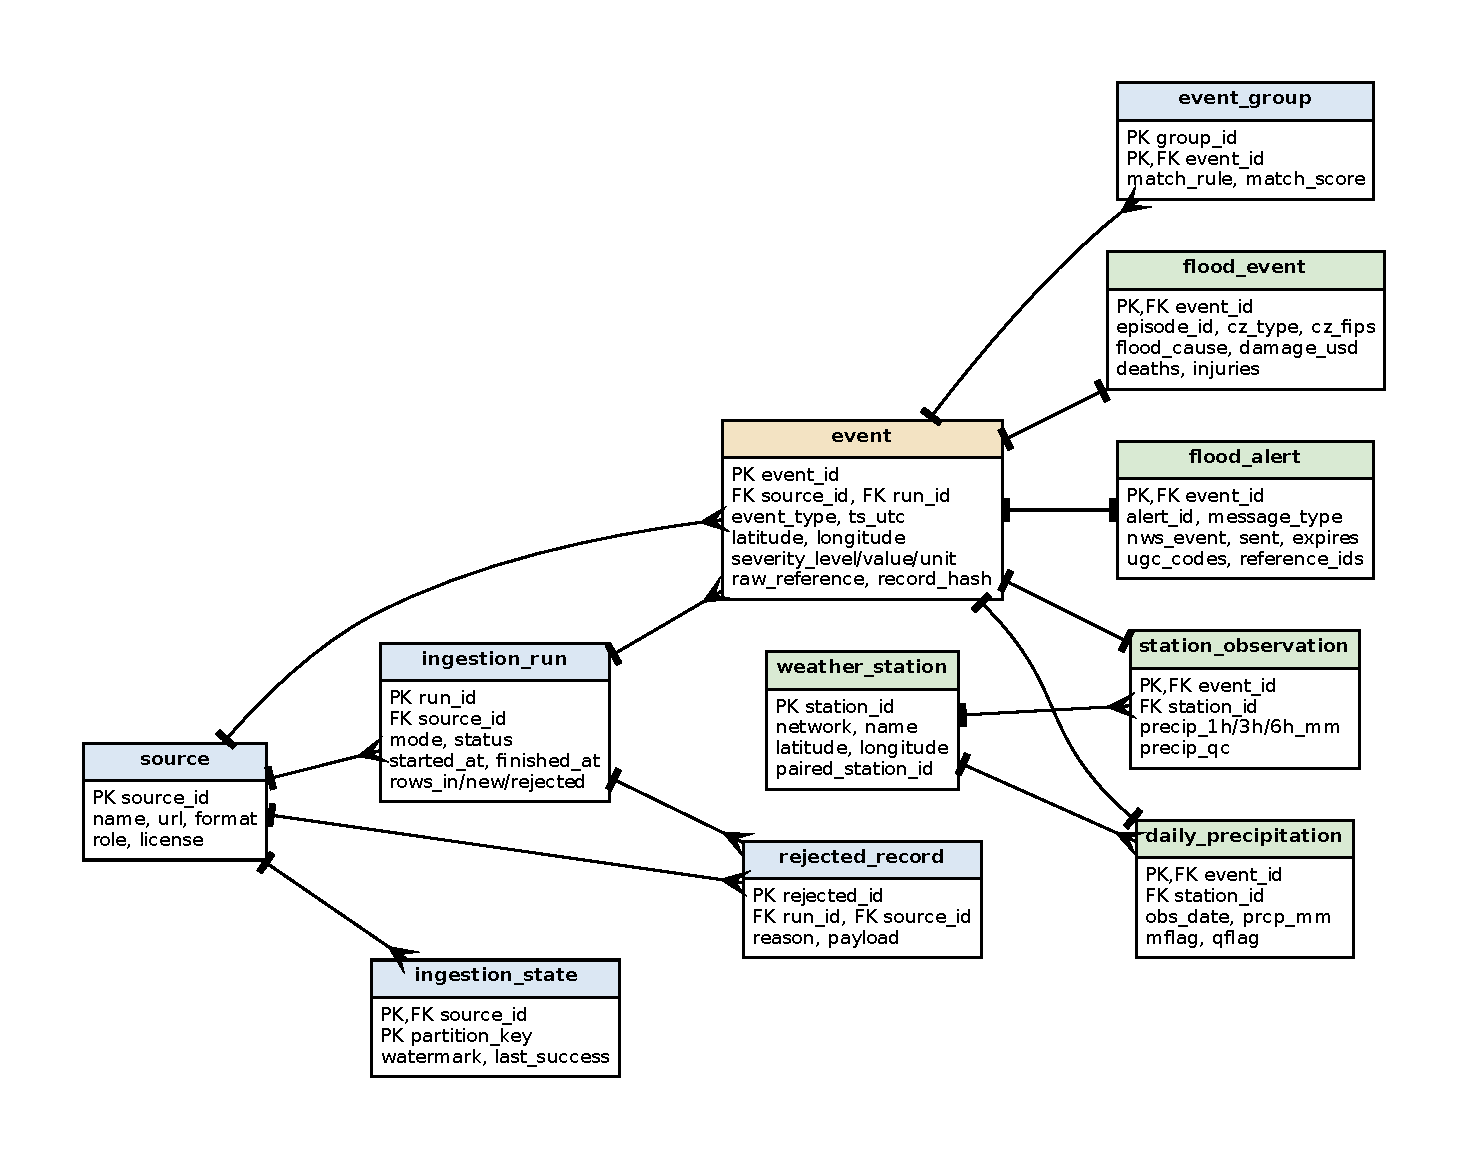
\includegraphics[width=0.95\textwidth]{figures/er_diagram.pdf}
\caption{First draft ER diagram: common model (blue), canonical event (orange) and flood domain tables (green).}\label{fig:er}
\end{figure}

% ===========================================================================
\section{Ingestion Contract (Draft)}
\begin{table}[H]\centering\small
\caption{Ingestion contract per source (details in \texttt{docs/ingestion\_contract.md}).}\label{tab:contract}
\begin{tabular}{@{}p{2.2cm}p{4.2cm}p{5.2cm}p{2.6cm}@{}}\toprule
Source & Historical strategy & Incremental strategy (watermark, frequency, overlap) & Duplicate key\\\midrule
Storm Events & Download each yearly file 2010--present once (cache), filter Texas + flood types; partition = year & Monthly listing check; watermark = \texttt{\_cYYYYMMDD} per year; changed suffix $\Rightarrow$ re-load that year; last 2 years always re-checked & EVENT\_ID\\
GHCN-Daily & One request per station $\times$ year (85 requests) & Daily; watermark = max DATE per station; re-request last 30 days & (STATION, DATE)\\
NWS observations & Load the $\sim$7 days the API keeps & Every 60 min; watermark = max timestamp per station; request from watermark $-$ 3~h & (stationId, timestamp)\\
NWS alerts & \texttt{/alerts?area=TX} with pagination for recent history & Every 15 min \texttt{/alerts/active?area=TX}; watermark = max \texttt{sent} + set of active ids; Update/Cancel chained by \texttt{references}; missing ids marked inactive & properties.id\\
\bottomrule\end{tabular}
\end{table}

\paragraph{Correctness when a run fails halfway.} Each run (i) stores raw responses in the landing zone first, (ii) loads and validates them, and (iii) upserts each partition (year, station-year or poll) \emph{in one transaction together with its watermark update}. A failure leaves finished partitions committed with their new watermark and the failed partition with the old one; the next run resumes from there. Because writes are upserts by the duplicate key, repeating a partition is idempotent. Invalid records go to \texttt{rejected\_record} with the reason and payload instead of stopping the run, and the run is recorded as \texttt{failed} in \texttt{ingestion\_run}.

% ===========================================================================
\section{Project Definition}

\subsection{Project overview}
\begin{itemize}
  \item \textbf{Title:} Flood Monitoring and Risk System for Texas.
  \item \textbf{Motivation:} flood information for Texas is spread across sources with different formats, time scales and geographic units (bulk CSV by county/zone, daily station totals, hourly observations, CAP alerts by forecast zone). Nobody can see in one place whether today's rain is unusual for a place with a history of flooding.
  \item \textbf{Goal (data engineering):} build a reproducible, idempotent pipeline that ingests two historical and two incremental sources into one canonical model, with watermarks, change detection, duplicate handling and quarantine. \textbf{Goal (analytics):} compare current rainfall and alerts with the historical rainfall distribution and flood frequency, and compute a Flood Risk Index per county.
  \item \textbf{Scope:} Texas; 2010--present; rainfall-driven flooding (Flood, Flash Flood, Heavy Rain); five paired stations, extendable through configuration.
  \item \textbf{Explicit exclusions:} no flood forecasting or hydrological modeling; no river-gauge (stage/discharge) data; no coastal storm-surge flooding; no real-time public warning service; no counties without a nearby station in the first version.
  \item \textbf{Constraints:} free and open sources only; NWS requires a User-Agent; Storm Events delay of several months; Docker Compose on a student laptop; three team members; four workshops.
\end{itemize}

\subsection{Functional user}
\textbf{Role:} emergency-management analyst at a Texas county or regional office (e.g., Harris County). \textbf{Profile:} follows the weather daily, knows NWS products, is not a programmer, needs answers in minutes. \textbf{Decisions supported:} raise internal readiness, pre-position resources or close low-water crossings, prioritize which counties to watch, and brief officials with evidence. \textbf{Why the dashboard helps:} it puts current rainfall, its historical rarity, past floods in the same county and active alerts on one screen, and states how fresh and complete each source is.

\subsection{User stories (MoSCoW)}
\begin{longtable}{@{}p{0.6cm}p{11.8cm}p{2cm}@{}}\toprule
ID & Story & Priority\\\midrule\endhead
US1 & As an emergency analyst, I want to see the flood alerts active now in Texas on a map so that I know where official warnings are in effect. & Must\\
US2 & As an emergency analyst, I want to see rainfall in the last 24 hours and 7 days per station so that I know where heavy rain is falling now. & Must\\
US3 & As an emergency analyst, I want current rainfall compared with the historical percentile for the same station and month so that I can tell whether it is unusual. & Must\\
US4 & As an emergency analyst, I want a Flood Risk Index (LOW/MEDIUM/HIGH) per county with the inputs that produced it so that I can prioritize counties and justify the decision. & Must\\
US5 & As an emergency analyst, I want to see when each source was last updated and how many records were rejected so that I know how fresh and complete the data is. & Must\\
US6 & As an emergency analyst, I want to see what is new since my last visit (new alerts, updates, cancellations) so that I do not miss changes. & Should\\
US7 & As a risk researcher, I want the historical flood frequency and damage per county since 2010 so that I can identify recurrently affected areas. & Should\\
US8 & As a risk researcher, I want to see which records from different sources were grouped as the same event so that I can trust the integration. & Could\\
US9 & As an emergency analyst, I want an e-mail notification when a county turns HIGH. & Won't (this semester)\\
\bottomrule\end{longtable}

\subsection{Indicator proposal: Flood Risk Index}
\textbf{Inputs} (per county, at time $t$): $R_{24}$ and $R_{7d}$, rainfall (mm) at the county's station; $P_{24}$, the percentile of $R_{24}$ in the station's historical distribution for the same month (GHCN-Daily 2010--present); $A$, the highest active NWS flood alert level (0 none, 1 advisory/statement, 2 watch, 3 warning); $F$, the historical flood frequency of the county (Storm Events flood records per year, 2010--present).

\textbf{Rule (preliminary):}
\begin{align*}
\text{rain\_level} &= \begin{cases} 3 & P_{24} \geq 99 \text{ or } R_{24} \geq 75\text{ mm}\\ 2 & P_{24} \geq 95 \text{ or } R_{7d} \geq 100\text{ mm}\\ 1 & P_{24} \geq 90 \\ 0 & \text{otherwise}\end{cases}\\
\text{score} &= \max(A, \text{rain\_level}) + \mathbb{1}[F \text{ in the top quartile of Texas counties}]
\end{align*}
\textbf{Output scale:} LOW (score 0--1), MEDIUM (2), HIGH ($\geq$3), shown together with its inputs and the freshness of each source. The index is a \emph{monitoring} aid, not a prediction of flooding.

\textbf{Validation against history:} alerts are not available for past years, so the rainfall + frequency part is back-tested with GHCN-Daily and Storm Events for 2010--present: for every county-day we compute the index and check (i) the share of Storm Events flood days classified MEDIUM/HIGH (hit rate) and (ii) the share of MEDIUM/HIGH days without any flood record (false-alarm rate). Thresholds are tuned on 2010--2020 and tested on 2021--present.

\subsection{Risks and mitigation}
\begin{longtable}{@{}p{3.5cm}p{5.5cm}p{5.8cm}@{}}\toprule
Risk & Impact & Mitigation\\\midrule\endhead
Source outage (NWS API down, NCEI maintenance) & Incremental runs fail; dashboard shows stale data & Retries with backoff; run marked failed and resumed from the watermark; freshness shown on the dashboard; recorded responses in \texttt{tests/fixtures} for development\\
Rate limits / blocked client & HTTP 403/429, missing data & Descriptive User-Agent, polling no faster than 15 min, cache all downloads, never re-download the archive\\
Schema change (new columns, API version, renamed file pattern) & Parsing errors & Schema validation before loading; unknown or invalid records to \texttt{rejected\_record}; source-status log and notice to the professor\\
Late revisions (Storm Events re-compiled, observations corrected) & Silent inconsistencies & Compile-suffix watermark per year; overlap windows; content hash per record\\
Ambiguous identifiers and locations (zone vs.\ county, alert chains, no shared key) & Wrong or missing event groups & UGC/FIPS lookup tables; matching rules with distance and time thresholds stored in \texttt{event\_group.match\_rule}; manual review of samples\\
Data volume / laptop resources & Slow loads, full disk & Texas and flood-type filtering at load; partitioning by year and station; raw files git-ignored\\
License / attribution & Non-compliance & All sources public domain; attribution recorded in \texttt{sources.yaml} and the report\\
\bottomrule\end{longtable}

\subsection{Architecture overview}
Figure~\ref{fig:arch} adapts the reference architecture of the course project \citep{sierra2026project}: sources $\rightarrow$ raw landing zone $\rightarrow$ normalize/validate/deduplicate $\rightarrow$ PostgreSQL/PostGIS (with quarantine) $\rightarrow$ analytics and indicator $\rightarrow$ Plotly Dash. Everything runs with Docker Compose; Apache Airflow schedules the incremental polls.

\begin{figure}[H]\centering
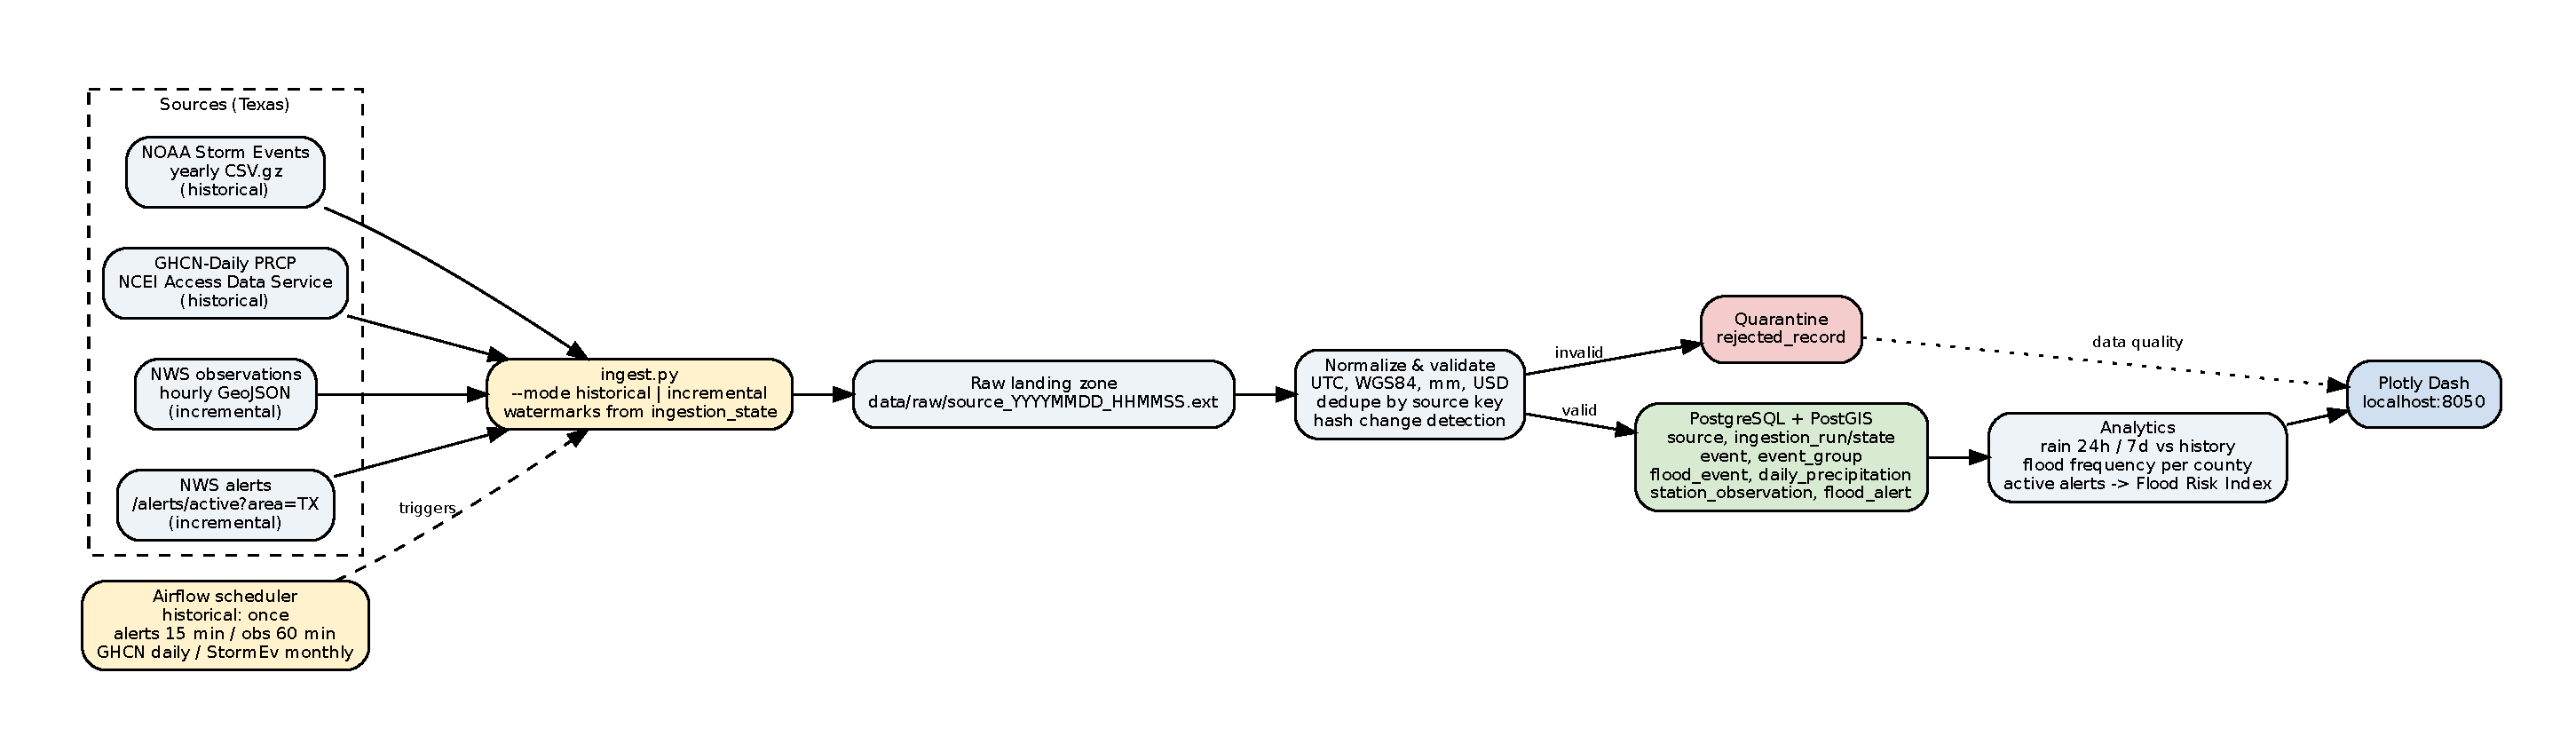
\includegraphics[width=\textwidth]{figures/architecture.pdf}
\caption{High-level architecture of the Flood Monitoring and Risk system.}\label{fig:arch}
\end{figure}

% ===========================================================================
\section{Repository}
Repository: \repo. Structure: \texttt{src/flood\_monitor/} (config, HTTP client, one module per source), \texttt{ingest.py} (CLI stub: \texttt{--mode historical | incremental | status}), \texttt{config/sources.yaml}, \texttt{data/raw/} (git-ignored), \texttt{sql/schema\_draft.sql}, \texttt{dashboard/}, \texttt{tests/} and \texttt{tests/fixtures/}, \texttt{notebooks/01\_source\_profiling.ipynb}, \texttt{docs/} (ingestion contract, ER and architecture diagrams, source-status log), \texttt{workshop\_1/} (\texttt{mapping.md}, \texttt{samples/}), \texttt{.env.example}, \texttt{.gitignore} and \texttt{README.md}. No secrets are committed: the NWS contact is read from \texttt{.env}. The large Storm Events yearly files are not committed; \texttt{scripts/fetch\_samples.py} downloads them into \texttt{data/raw/}.

\bibliography{references}

\end{document}
